\chapter{Optimal Pricing on Networks under Partition Constraints}\label{ch:pricing}

% Write-up window in the plan: Oct 5 -- Oct 18.
% If this chapter is based on a paper, start by pasting the paper in and
% then (1) remove the paper's own intro/lit review overlap with Ch. 1,
% (2) switch notation to the macros in thesis.sty, (3) fix \cref labels.

\section{Introduction}\label{sec:pricing:intro}

		Using social network information to harness peer effects has been an active research topic in recent years. Network effects shape critical outcomes in a social network such as the spread of information, ideas and disease (see, e.g.,~\cite{banerjee2013diffusion},
~\cite{pastor2001epidemic},
~\cite{muchnik2013social},
~\cite{chamley2004rational}), adoption of products (see, e.g.,~\cite{bapna2015your, rogers1976new, wang2016consumer}) among others.

	Our work is related to the broader literature on positive network externalities~\cite{farrell1985standardization},~\cite{katz1985network} and in particular to marketing with positive network
	externalities. This literature is categorized in two streams. The first stream aims at maximizing adoption through {\it influence maximization} and the second stream aims at {\it revenue maximization} through pricing decisions.
	
 Influence maximization initially introduced in~\cite{domingos2001mining} aims at identifying the best {\it seeds} to trigger cascades of influence that maximize the overall spread of influence and adoption in the social network. Subsequent literature has studied influence maximization in various settings, see, e.g.,~\cite{richardson2002mining} and~\cite{banerjee2013diffusion}.~\cite{kempe2003maximizing} showed that this problem is computationally hard, but approximation
	algorithms provide good performance with provable guarantees. Recent work~\cite{akbarpour2018} studied 
	the value of network information for influence maximization and showed that for a class of random networks, random seeding strategies with a few more seeds can lead to  larger cascades than optimal seed selection. Follow up work~\cite{Jackson-Storms-2017} has showed that this may not be the case for all networks and uncertainty structures. This follow up work is in the spirit of our work.
	
	Our work mainly belongs to the revenue maximization stream. Revenue maximization problems aim at maximizing the revenue through pricing. There has been much research using pricing under
	network effects in
	the setting of sequential purchase decisions
	(see, e.g.,~\cite{hartline2008optimal},~\cite{arthur2009pricing},
~\cite{haghpanah2013optimal},~\cite{crapis2016monopoly},~\cite{zhou2018optimal}) and
	simultaneous purchase decisions (see, e.g.,~\cite{campbell2013word},
~\cite{du2016optimal},~\cite{chen2018competitive},~\cite{cohen2013designing}). Such
	problems are often computationally hard and most literature focuses
	on the computational  aspect.
	
	Our work is closely related to the static pricing problem of selling
	a divisible product to a group of consumers with positive network
	externalities, in particular, the works of~\cite{huang2019value},~\cite{huang2022value},\cite{candogan2012optimal},~\cite{bloch2013pricing} and~\cite{fainmesser2015pricing},~\cite{Baron-2022}. In particular, we build upon the model in~\cite{huang2022value}. These
	works consider a two-stage game, in which the merchant first
	chooses the prices and then the consumers, embedded in a social
	network, make purchasing decisions simultaneously.~\cite{candogan2012optimal} and~\cite{bloch2013pricing} assume full network information, while~\cite{fainmesser2015pricing},~\cite{Baron-2022},\cite{huang2019value}, and~\cite{huang2022value} assume incomplete network information. In
	these works, prices can be set differently based upon consumers'
	positions in the social network. The question of interest in~\cite{candogan2012optimal},~\cite{bloch2013pricing} and~\cite{fainmesser2015pricing} is to
	characterize and identify optimal prices and profits in the networks
	and the complexity of computing optimal prices. In contrast,~\cite{huang2019value},~\cite{huang2022value} quantify the value of network information for pricing in Erd\"{o}s-Renyi random networks and Power-law networks under configuration model. Their results show that in such networks the value of network information vanishes asymptotically in the size of the network. Our work is the first to show that there exists a class of random networks (with community structure that persists asymptotically) for which the value of network information does not vanish asymptotically. Further, our work is the first to show that in such networks, the merchant does not need the full network information and the community structure and membership  information is sufficient to derive near optimal profit, thus establishing that the community information is very valuable while the rest of the information about the network may not have much value.
	
	Moreover, in developing the asymptotic value
	of network information in random networks, we find connections
	with graph theory and random graph theory, in particular, the literature on counting
	the number of walks of different lengths in a network
	(see, e.g.,~\cite{fiol2009number},~\cite{levin2017counting}), on spectral
	graph theory (see, e.g.,~\cite{krivelevich2003largest},~\cite{chung2004spectra},~\cite{preciado2017moment}), and on
	network centrality (see, e.g.,~\cite{bonacich1987power}).


\section{Model}\label{sec:pricing:model}
In this section, we introduce the preliminary model for the merchant and the agents. We study a firm selling a divisible good to agents embedded in a directed social network. The network is represented by a matrix $G \in \mathbb{R}^{n\times n}_{+}$ where $G_{ij}$ is the influence the $j$th consumer has on the $i$th.   The merchant first sets prices, and then each consumer chooses how much to purchase as a function of their position in the network and the price charged. The consumers all make a single purchasing decision simultaneously. 

  
\subsection{Consumer utilities}
Each agent, $i$, consumes an amount of the good, $x_i$, to maximize their own personal utility, $u_i$. Let $\tb{x},\tb{u}$, and $\tb{p}$ denote the vectors of consumption, utility, and price, respectively. Utility depends on one's consumption, the price they are charged, and the consumption of peers. This network externality incorporates the impact that social connections have on consumption. As one's peers consume more, the marginal   utility of consuming more increases.  In full, the utility function for the ith individual is 
\[u_i(x_i, \mathbf{x}_{-i}, p_i) = ax_i - p_i x_i - x_i^2 + 4\rho x_i \sum_{j\neq i} \frac{G_{ij}}{\| G +G^T\|}x_j .\]

Here, $a>0$ and $\rho \in (0,1)$ are constants. $a$ represents the utility gained from obtaining the first unit of the good, and $\rho$ represents the strength of the network externality effect.  The scaling factor $\frac{1}{\|G+G\|}$ ensures that the model has well-defined solutions as described below. 

In this model, each agent will purchase an amount to maximize their own personal utility. But this decision requires knowing how much their peers are consuming, and the peers need to know how much their peers are consuming.  This is a network game and has been shown to have a unique equilibrium. 

\begin{proposition}[Unique Equilibrium~\cite{candogan2012optimal}, eq. 5]
    When the merchant charges the users $\textbf{p}$, there is a unique equilibrium consumption of the form:
    \begin{equation}
        \mathbf{x}^*(\bp) = \frac{1}{2} {\left(I - 2\rhof G\right)}^{-1} (a\bo - \bp) 
    \end{equation}
\end{proposition}


The expression $ {\left( I - 2\rho\frac{G}{\|G + G^T\|}\right)}^{-1} $ is well-defined and exists because $2 \rho \frac{G}{\| G +G^T\|}$ has all of its eigenvalues with magnitude between 0 and 1. Therefore, this matrix will have a well-defined inverse~\cite{fan1949theorem}. The term ${(I - 2\rhof G)}^{-1}$ can be expanded as $\sum_{k=0}^\infty {\left(2\rhof\right)}^k G^k$, and this expansion provides more insight into what this term says about how the network structure determines consumption. The ij-th element in the kth term of this series represents the number of walks of length exactly k from i to j discounted by a factor of ${\left(2 \rhof\right)}^k$. 

\subsection{Optimal Pricing}
The problem of the merchant is to maximize the profit under this consumption model. The profit from consumer $i$ is how much they consumed times the net profit per unit for that individual. The net profit per unit is $p_i - c$, where $a>c>0$ is the cost per unit of production. The total profit is the sum over the profit from each individual. In summary, the problem is 
\begin{equation}
    \max_{\bp} \frac{1}{2} {(\bp - c \bo )}^T \mathbf{x} (\bp) 
\end{equation}

This problem has an explicit solution given below. 
\begin{proposition}[Optimal Price,~\cite{candogan2012optimal} Theorem 3]
    With a cost of production c, the profit-maximizing price vector is:
    \begin{align*}
        \bp^* &= %\frac{a+c}{2} \bo + \frac{a-c}{2} \rhof G^T \left(I - \rhof (G+G^T)\right)^{-1} \bo \\
        %&- \frac{a-c}{2}  \rhof G \left(I - \rhof (G+G^T)\right)^{-1} \bo \\
         \frac{a+c}{2} \bo  + \rhof \frac{a-c}{2}  (G-G^T) {\left(I - \rhof (G+G^T)\right)}^{-1} \bo
    \end{align*}

    This price yields the optimal profit, $\Pi^*$ of:
    \begin{equation}\label{eq:opt_prof}
        \Pi^* = \frac{{(a-c)}^2}{8} \bo^T {\left(I - \rhof (G+G^T) \right)}^{-1} \bo
    \end{equation}
\end{proposition}

The expression of the price looks complicated but can be broken down into three parts. The first part represents a common term that everyone is charged. The second term is a markup that a consumer is charged for being influenced in the network, and the third term is a discount for being influential in the network. A consumer will frequently be both the influenced and the influencer. These markup and discount terms are based on the expression ${\left(I - \rhof (G+G^T) \right)}^{-1} \bo$, the Bonacich centrality vector. This is another weighted sum of walks in a network, but now $G+G^T$ is used, while the consumption in the network was based on $2G$. The optimal profit is proportional to the sum over all centrality of all nodes. Equation~\ref{eq:opt_prof} says that the optimal profit is proportional to the weighted sum of walks in the network $G+G^T$. 

\subsection{Regret}

In this chapter, we will study how well different pricing strategies compare to each other. To formally study these questions, we introduce the notions of regret and fractional regret consistent with previous work~\cite{huang2022value}. 

\begin{definition}
    The regret of a price vector $\bp$ compared to $\tb{q}$ is $Regret(G, \tb{p}, \tb{q}) \defeq \Pi(\tb{q}) - \Pi(\bp)$ where $G$ is the underlying network of $\Pi$.
\end{definition}

Although this is the most natural notion of regret, an additive measure of regret breaks down as we work on networks with different topologies and sizes. A regret of  $\$10,000$ could be a small loss or a catastrophic loss and without proper context it is not clear how to tell. Instead, we will often choose to ask what fraction of the possible profit is lost with the fractional regret. 

\begin{definition}
    The fractional regret of a price vector $\tb{p}$ compared to $\tb{q}$ is $Regret_F(G, \tb{p}, \tb{q}) \defeq 1 - \frac{\Pi(\bp)}{\Pi(\tb{q})}$
    where G is the underlying network of $\Pi$.
\end{definition}

We will frequently care about these notions of regret when comparing to the optimal price $\tb{p}^*$ and will make it clear when this is not the case.  In particular, we will say a price $\tb{p}$ has zero-regret or is regret free if the regret of $\tb{p}$  compared to $\tb{p}^*$ is zero. 


A core question that this paper studies is what pricing schemes asymptotically have zero fractional regret for a sequence of random graphs, and what level of information is required to achieve such pricing schemes? If the fractional regret under uniform pricing goes to zero, then information of the network is not valuable. For this reason, the fractional regret of uniform pricing can be treated as the value of information. When the merchant can expect nearly the same profits without needing to learn the network, they are better off not expending the effort to do so. Below is a formal definition of what it means for the fractional regret to go to zero compared to the optimal price in the limit as the network size increases.


\begin{definition}
    We say that a sequence of networks $\{G_n\}$ is "regret-free with respect to a pricing scheme $\tb{p}_n$"  if for any $\epsilon > 0$ there is a number $n_0$ such that for all $n > n_0$
    \begin{equation*}
        \ev{ Regret_F(G_n, \tb{p}_n, \tb{p}_n^*) } < \epsilon
    \end{equation*}

    Where $\tb{p}_n^*$ is the optimal price
\end{definition}

In recent work, \cite{huang2022value}, have shown that for a large class of networks, including Erd\"{o}s-Renyi graphs and Power-Law networks, the value of information goes to zero almost surely in the size of the network. Whether there exists a class of random graphs for which the fractional regret does not asymptotically vanish was an open question. Here we answer this question definitively by showing classes of random networks where the value of information is non-zero. 

Throughout this work we will look at networks with a density of $\Omega( \frac{\log n}{n})$ because \cite{huang2022value} also showed that when random networks are sparser, the network effect will be weak and make up a small portion of the total profit leading to asymptotically zero regret for uniform pricing.


\subsection{The Stochastic Block Model}
Now that we have developed the framework for studying regret under very general structures, we apply these methods to a particular case, the stochastic block model or SBM when it is clear.  We consider a stochastic block model, a generative random graph model, with nodes partitioned into $m$ communities each of size $n$ for a total of $mn$ total nodes. Nodes in the same community behave in a statistically independent and identical way. The probability of connection between two nodes is determined at the block-level. If a and a' are two nodes in community i and b and b' are two nodes in community j then $\Pr(\text{a has an edge to b}) = \Pr(\text{a' has an edge to b'}) = M_{ij}$ independent of the existence or non-existence of any other edge. We can collect this information into one $m \times m$ matrix M where $M_{ij}$  is the probability of connection from community i to j. We will call such a matrix the community structure matrix or the block matrix. This matrix is allowed to have diagonal entries and can be asymmetric.  


This structure is random but due to the strong community structure there is a natural pricing strategy to use beyond uniform and optimal pricing. The merchant may use the community structure as a basis for pricing. That is, they set one unique price for all nodes belonging to the same community. One reason to do this is that it requires less information than the full optimal pricing. The amount of information required is given by the following proposition. required is given by the following proposition. 
\begin{proposition}
        Optimal block-level pricing uses full community information and requires a total of  $\Theta ( m^2 + nm )$ entries be known. 
    
    The full network information requirement for using optimal pricing is $\Theta( n^2 m^2 )$.
\end{proposition}

The information requirement for the optimal pricing is $\Theta(n^2 m^2)$ entries because it requires knowledge of the full adjacency matrix. Optimal pricing requires the complete adjacency matrix, which has $nm \times nm$ entries. Optimal block-level pricing requires the knowledge of community structure matrix, which has $m \times m$ entries and an additional $mn$ entries to track what community each node belongs to. We will store this community membership information into a matrix $R \in \mathbb{R}^{m \times nm}$ where $R_{ij} = \begin{cases} 1 & \text{ j in community i} \\ 0 & \text{ else} \end{cases} $.

Using this pricing strategy and given the community information, the optimal block-level price, $\tb{p}_{comm}$ is given by the following theorem. 
% \am{$B$ has been used earlier.}
\begin{theorem}\label{prop:group_pricing}
    Using the communities defined by $R$, the optimal block-level price is given by:
    \newcommand{\D}{D}
    \begin{equation*}
        \tb{p}_{comm} = R^T \left( R (D+D^T) R^T\right)^{-1} R (a D + cD^T) \one 
    \end{equation*}
    where $D = \left( I - \frac{2\rho M}{\| M+M^T\|}\right)^{-1} \otimes I_{n,n} $ and $\otimes $ is the Kronecker product operator.
\end{theorem}

 In many cases the community information is readily available to the merchant because of the user profile information. In other cases, stochastic block models, the community structure can be inferred from the partial and noisy observation of the network. To answer how good this pricing strategy is and how valuable the community information is, involves answering two questions.
\begin{enumerate}
    \item \emph{Does pricing using the optimal uniform pricing have non-vanishing regret?} If the answer to this question is yes then there is some value to network information. In that case the next question becomes relevant.
    \item \emph{Does pricing using just block information lead to an asymptotically low regret solution?}
\end{enumerate}
The second question asks if this level of information is sufficient for low regret pricing. Our next step is answering these questions by showing having the granular view of only the community information in the network is sufficient and ignoring the network structure in determining prices is insufficient. However, when the network is too sparse, the value of the network information is already too small because the network effect it weak as shown in \cite{huang2022value}. For this reason we study a regime where the network is sufficiently dense meaning that the probability of connections scales at a rate of at least $\frac{\log(n)}{n}$.  
%If the uniform pricing is insufficient to get a good solution, then more information about the network is needed. Answering both of these questions for the stochastic block model will tell us that some information of the network is necessary and sufficient to get a low regret solution. 

The expected profit under optimal block-level pricing is given below.

\begin{theorem}\label{thm:sbm_opt}
    Let $G_n$ be a sequence of SBMs with community structure $M$ with density $p(n) = \Omega\left(\frac{\log (n)}{n}\right)$. 
    The asymptotic expected profit under optimal block-level pricing is
    \begin{align*}
        &\ev{\bo^T \left(I - \frac{2\rho}{\|G+G^T\|}  G\right)^{-1} \bo}\\
        &+ \left(\frac{\rho}{p(n) n \|M+M^T\|} \right)^2 \ex{ \bo^T (G^T-G)(G-G^T)\bo} + o\left( \left( p(n) n \|M+M^T\| \right)^{-3} \right)
   \end{align*}
\end{theorem}
This particular form of the profit decomposes into three pieces based on the series expansion of the profit. The first term is the expected profit under optimal uniform pricing. The second term is the remainder of the low-order terms of the series expansion of the profit, and the third term represents the higher-order terms, which are small as compared to the first- and second-order terms as the walks are weighted geometrically by their length. Specifically, the expression in the second $\ev{\bo^T (G^T - G)(G-G^T) \bo}$ is the sum of the expected quadratic difference between the out-degree ($out_i$) and in-degree($in_i$) (the uncentered second moment) over all nodes. In other words, this is $\sum_{i=0}^{nm} E[ (in_i - out_i)^2]$.   As a corollary to Theorem \ref{thm:sbm_opt}, we obtain the regret under using uniform pricing compared to optimal pricing.

\begin{corollary}
    \label{cor:uni_sbm_reg}
    Consider a sequence of SBMs using community structure M with density $\Omega(\frac{\log(n)}{n})$. Then the expected regret of uniform pricing is:
    \begin{equation}
        \left(\frac{\rho}{p(n) n \|M+M^T\|} \right)^2 \ex{ \bo^T (G^T-G)(G-G^T)\bo} + o\left( \left(p(n) n \|M+M^T\| \right)^{-3} \right)
    \end{equation}
\end{corollary}

The proof follows by noting that the first term of Theorem \ref{thm:sbm_opt} corresponds to the profit under uniform pricing. This corollary implies that the expected regret under uniform pricing grows linearly with the number of nodes per community. This is due to the fact that the uncentered second moment grows at a rate of $\Theta(n^2 p(n)^2)$. Summing over all the nodes of the network, we find that the numerator of this expected regret is $\Theta(n^3 p(n)^2)$ and is normalized by $\frac{\rho^2}{ (p(n) n \|M+M^T\|)^2 }$, which leaves us with a regret that grows like $\frac{\rho^2 n }{\|M+M^T\|^2}$. This means we expect the regret from using uniform pricing to not vanish. 

In contrast, the block-level pricing yields the following profit.  
\begin{theorem}\label{thm:sbm_block}
    Let $G_n$ be a sequence of SBMs with community structure $M$ with density $\Omega(\frac{\log (n)}{n})$. As the size of communities grows to infinity, the asymptotic expected profit under optimal block-level pricing using full community information is:
        \begin{align*}
        &\ex{ \bo^T \left(I - 2\rhof G \right)^{-1} \bo}  \\
        &+ \left(\frac{\rho}{p(n) n \|M+M^T\|}\right)^2  \bo^T ( \ev{G^T}-\ev{G})(\ev{G}-\ev{G^T})\bo + o( (p(n) n \|M+M^T\|)^{-3} )
    \end{align*}
\end{theorem}

This is obtained by expanding the series representation of the profits and separating terms into the uniform profit, first- and second-order terms, and higher-order terms.  In Corollary \ref{cor:uni_sbm_reg}, the additive part of the regret is equal to the sum of the second moments of the difference in degree and out-degree of each. In parallel to the uniform case, here the additive part can be expressed as the square of the expectation of the out-degree minus in, $\sum_{i=0}^{mn} (\ev{out_i} - \ev{in_i})^2$. Therefore the regret under block-level pricing using full community information, this can be written in terms of the variance of the in-degree and out-degree. 
\begin{theorem}\label{prop:var_expression}
        Let $G_n$ be a sequence of SBMs with community structure $M$ with density $\Omega(\frac{\log (n)}{n})$. As the size of communities grows to infinity, the expected regret from optimal block-level pricing using full community information is:
    \begin{equation}
        \frac{ n \rho^2}{ (n p(n) \|M+M^T\|)^2 } \sum_{i =1 }^{m} Var( in_i ) + Var(out_i)   + o\left( \left(n p(n) \|M+M^T\|\right)^{-3}\right),
    \end{equation}
    where $in_i, out_i$ is the random variable of in(out)degree for community  i
\end{theorem}

The variance of the in and out degree grows slower than the uncentered second moment, at a rate of $n p(n)$, but is still normalized by $\frac{1}{n^2 p(n)^2 \|M+M^T\|^2 }$. This means that the expected regret from using the full community information grows sublinearly in the number of nodes per community. A sublinear growth in the expected regret is sufficient to conclude that the expected fractional regret goes to zero as $n \to \infty$. 



%\subsection{Methods}
\subsection{Proof techniques}  To establish these results, we need to characterize the distribution of the spectral norm of $\|G+G^T\|$. The following Lemma states that asymptotically almost surely, this norm is close to the norm of M scaled by a factor of n. 

\begin{lemma}\label{lem:norm_eq}
    Consider a sequence of SBMs with structure M with density $p(n) = \Omega(\frac{\log n}{n})$. Then $\|G+G^T\| = p(n) \left(1+ o(1)\right) n \| M+M^T\| $ asymptotically almost surely, where n is the nodes per community 
\end{lemma}
A proof may be found in Appendix \ref{proof:norm_eq}. Suppose that $\mathbf{u}$ is the largest eigenvector of $M+M^T$ with $(M+M^T) \mathbf{u} = \lambda_n$. The proof then shows that the growth of the largest eigenvalue of $G+G^T$ is governed by the number of nodes per community, their density, and $\lambda_n$. An important part of this proof is that largest degree and the average degree grow like $p(n) n d_{max}(M+M^T)$ and $p(n) n d_{ave}( M+M^T)$ where $d_{max}(M+M^T)$ is the largest degree of $M+M^T$ and $d_{ave}(M+M^T)$ is the average degree. This provides an upper and lower bound on the largest eigenvalue of $G+G^T$.

Additionally, another key aspect of the proofs of this section involves expanding the inverses that make up the prices and profits via the series expansion $(I - A)^{-1} = \sum_{k=0}^\infty A^k$.  From this series expansion,  we isolate the term corresponding to uniform pricing. In Theorem~\ref{thm:core_regret} and Theorem~\ref{thm:core_regret_uni} the first order terms vanish in expectation because they are linear. The terms with order higher have a limited impact on the regret because the weight of long walks decays exponentially in the length of the network. 
% \am{This is abrupt.} There are three prices and their respective profits and regrets to consider: the optimal price with full network information, the uniform pricing with no network information required, and the optimal pricing using the block-level information. First, we discuss the gap from uniform pricing and follow it with a discussion of the performance of using block-level information. 


\subsection{Example: The Tree Model}
Here, we show an example to demonstrate the value of the community information. We consider a special case where the community structure M takes the form of a directed tree with weights $p(n)$. We will refer to this as the tree-SBM model. To form a Tree-SBM of height h, branching factor $b$, with $n$ nodes per community density $p(n)$  we do the following two steps:
\begin{enumerate}
    \item Let $M$ be the adjacency matrix of a tree with branching factor $b$ and height $h$ with edges directed from towards the the leaf node. 
    \item Generate $G$, an $SBM$ matrix with n nodes per community with a community structure of $p(n) M$
\end{enumerate}


This network has a strong asymmetric structure, which means some communities are more influential than others and that we should expect uniform pricing to be a poor choice. This exercise first works to showcase the differences in uniform and block-pricing in the SBM model. But beyond this first goal, we will use the simpler structure to motivate our later study of general uncertainty structure.

Here, we state the theoretical results of the regret from block-level pricing. 

\begin{theorem}\label{thm:core_regret}
    Let $\{G_n\}$ be a sequence of SBMs with a tree community structure with a branching factor of $b$ and density $p(n) = \Theta( \frac{\log n}{n})$. Then the expected regret from block-level pricing is $\Theta\left(\frac{\rho^2 b^{h}}{ p(n)}\right)$.

    Furthermore, the fractional regret goes to $0$.
\end{theorem}

This theorem follows by applying Theorem \ref{prop:var_expression} and bounding the spectral norm of $\|G_n +G_n^T\|$. A full proof may be found in Appendix \ref{proof:core_regret}. This result states that the regret from using block-level pricing grows sublinearly, and there is vanishing fractional regret. Using only the block-level information as opposed to the individual edges is sufficient. The regret for optimal uniform pricing for this network is given by the following Theorem.

\begin{theorem}\label{thm:core_regret_uni}
   Let $\{G_n\}$ be a sequence of SBMs with a tree community structure with a branching factor of $b$ and density $p(n) = \Theta( \frac{\log n}{n})$. Then the expected regret from optimal uniform pricing is $\Theta\left(\frac{b^{h+1} -1 }{b-1} n \rho^2\right)$

    And the fractional regret converges to a constant $0<c<1$. 
\end{theorem}

The proof follows from Corollary \ref{cor:uni_sbm_reg} and by bounding the spectral norm of the adjacency matrix. Details may be found in the Appendix \ref{proof:core_regret_uni}. For both of these results, the $b^h$ is not prohibitive as it appears. This term shows up because the total number of communities is $\frac{b^{h+1} - 1}{b-1}$ and regret for both of these pricing strategies scales with the total number of communities. Theorem \ref{thm:core_regret_uni} states that no information is insufficient for good performance. The reason for the difference is due to the differing growth rates of $Var(in), Var(out)$ for block pricing and $\ex{in^2}, \ex{out^2}$ for uniform pricing. In the variance expression, the highest-order terms cancel out. 

One might wonder what happens if this community structure loses its sharpness. How much noise can the model take while still having the same asymptotic bounds? To explore this, we consider adding $\S$ random edges to a tree SBM network. As the number of random edges increases, the network becomes more and more uniform, and the discrepancy between the most and least central nodes will decrease.  We should expect that there is a threshold of noise where doing block-level pricing does not earn us an advantage over uniform pricing. We establish a clear threshold function for regret of using uniform pricing. 


\begin{theorem}\label{thm:noise}
    Let $\{G_n\}$ be a sequence of SBMs with a tree community structure with a branching factor of b and a density of $p(n) = \Theta \left( \frac{ \log(n)}{n} \right) $ with $\S$ random edges added. Then the expected regret from optimal uniform pricing is:
    \begin{equation}
       \begin{cases} 
        \theta(n) & \text{ if } \S = o(n \log n) \\ 
        o(n) & \text{ if } \S = \omega (n \log n)
        \end{cases}
    \end{equation}
\end{theorem}
A proof may be found in the Appendix ~\ref{proof:noise} 

This result shows that only when the noise is very large, enough to overwhelm the network effect only then there is no value to information of the network. The robustness makes using this framework much more appealing, as even when the network changes or the measurements of the community structure are noisy, the merchant can expect the results to still hold. In particular, the regret is characterized by a threshold function where if the number of random edges grows below a certain rate, the fractional regret of uniform pricing goes to 0, and when K grows faster, the fractional regret goes to a positive constant. 
 
% One way to conceptualize this result is that there are two competing forces: the network asymmetry and the homogenizing effect of the addition of random edges. The result shows that what matters more is determined by what is more prevalent asymptotically. Important to this conclusion is that the spectral norm will be controlled by the more common component.  
\subsubsection{Numerical Simulation}
\begin{figure}
    \centering
    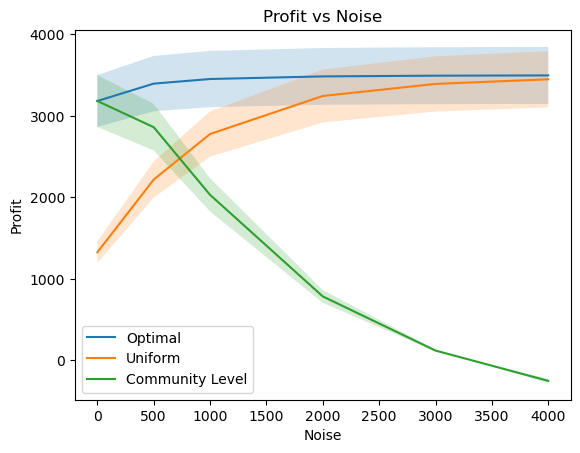
\includegraphics[width=0.45\linewidth]{Figures/Pricing/sbm.png}
    \caption{Profits vs noise for the Tree-SBM model for three pricing strategies. Blue is the optimal profit, orange is the uniform profit, and green is the profit using block-level pricing. }
    \label{fig:sbm}
\end{figure}

Here, we show the validity of the results in this section through numerical simulation. We will simulate an SBM with a tree structure as the size of communities and the amount of noise added change. We use a tree of height 3 with 100 nodes per community.  What we see in Figure \ref{fig:sbm} is that when the noise is low, using community information does well and suffers negligible losses, while a large fraction of profits are lost using the uniform pricing. But what we see is that as the noise increases, the uniform pricing increases profit. This is because there are more total edges, so the weighted sum of walks is higher, which the uniform pricing captures. But the profits from using the block-level information decrease. This is because the differences in centrality that the block-level price hoped to capitalize on are increasingly incorrect and mismatched with the optimal price. 

There is a gap in Theorem $\ref{thm:noise}$. When the amount of noise and the amount of structure are balanced and grow at the same rate, it is unclear what the behavior should be. In the next section, we address this and study a setting where the amount of noise is a fraction of the total network.





